$$
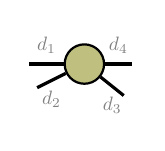
\begin{tikzpicture}[baseline=-0.5ex]
    \tikzset{tensor/.style = {minimum size = 0.5cm,shape = circle,thick,draw=black,inner sep = 0pt}, edge/.style = {thick,line width=.4mm},every loop/.style={}}
    \def\x{6}
    \def\y{0}
     \node[tensor,fill=green!50!red!50!white] (B) at (\x+1,\y) {$\St$};
    \draw[edge] (B) -- (\x+0.3,0) node [midway,above] {\scalebox{0.7}{\textcolor{gray}{$d_1$}}};
    \draw[edge] (B) -- (\x+1.6,0) node [midway,above] {\scalebox{0.7}{\textcolor{gray}{$d_4$}}};;
    \draw[edge] (B) -- (\x+0.4,-0.3) node [midway, below] {\scalebox{0.7}{\textcolor{gray}{$d_2$}}};;
    \draw[edge] (B) -- (\x+1.5,-0.4)node [midway, below] {\scalebox{0.7}{\textcolor{gray}{$d_3$}}};;
\end{tikzpicture}=
\begin{tikzpicture}[baseline=\baseline]
    \tikzset{tensor/.style = {minimum size = 0.5cm,shape = circle,thick,draw=black,inner sep = 0pt}, edge/.style   = {thick,line width=.4mm},every loop/.style={}}
    \def\y{0}
    \def\x{0}
  \node[tensor,fill=red!30!white] (D) at (\x-1,\y){$\Gt_1$};
  \node[tensor,fill=red!50!white] (A) at (\x,\y){\scalebox{0.85}{$\Gt_2$}};
  \node[tensor,fill=blue!50!white] (B) at (\x+1,\y){$\Gt_3$};
   \node[tensor,fill=blue!20!white] (C) at (\x+2,\y){$\Gt_4$};
    \draw[edge](A) -- (\x,\y-0.7)node [midway,left] {\edgelabel{$d_2$}};
    \draw[edge](B) -- (\x+1,\y-0.7)node [midway,left] {\edgelabel{$d_3$}};
    \draw[edge](C) -- (\x+2,\y-0.7)node [midway,left] {\edgelabel{$d_4$}};
     \draw[edge](D) -- (\x-1,\y-0.7)node [midway,left] {\edgelabel{$d_1$}};
    \draw[edge](D) -- (A) node [midway,above] {\edgelabel{$R_1$}};
    \draw[edge](A) -- (B) node [midway,above] {\edgelabel{$R_2$}};
    \draw[edge](B) -- (C) node [midway,above] {\edgelabel{$R_3$}};
\end{tikzpicture}.
$$
TT 分解最早在量子物理与凝聚态物理社区中以 \emph{矩阵乘积态}（Matrix Product States, MPS）之名提出。在这一语境下，内部边的维数被称为 \textit{键维数}，自由腿则称为 \textit{物理维数}。
接下来我们说明如何在多项式时间内，利用逐次奇异值分解（SVD）计算张量 $\St\in\RR^{d_1\times\dots\times d_N}$ 的精确 TT 分解。该算法被称为 TT-SVD 算法~\citep{oseledets2010approximation}，但更早由量子物理社区引入，并被称作 \textit{逐次 Schmidt 分解}~\citep{vidal2004efficient,mcculloch2007density}。
在给出 TT-SVD 算法之前，先介绍三阶张量的左正交与右正交概念。
\begin{definition}\label{def:left-right-ortho}若 $(\At_n)_{(3)}^\ts(\At_n)_{(3)}=\Ib_{R_n}$，则称 $n\in[N]$ 对应的核心张量 $\At_n\in\RR^{R_{n-1}\times d_n\times R_n}$ 左正交；若 $(\At_n)_{(1)}(\At_n)_{(1)}^\ts=\Ib_{R_{n-1}}$，则称其右正交。这可以用张量网络
图示如下：
\begin{align*}
\begin{tikzpicture}[baseline=\baseline]
    \tikzset{tensor/.style = {minimum size = 0.5cm,shape = circle,thick,draw=black,inner sep = 0pt}, edge/.style = {thick,line width=.4mm},every loop/.style={}}
    \def\y{0}
    \def\x{0}
    \node[tensor, path picture={
    \fill[fill=red!30!white](path picture bounding box.south east)
        -- 
    (path picture bounding box.north west) --
    (path picture bounding box.north east) -- cycle;
    }, shift={(\x,\y)}] (A) {\scalebox{0.85}{$\At_n$}};
    \draw[edge](A) -- (\x,\y-0.7)node [midway,left] {\scalebox{0.7}{\dimcolor{$d_n$}}};
    \draw[edge](A) -- (\x-0.85,\y)node [midway,above] {\scalebox{0.7}{\dimcolor{$R_{n-1}$}}};
    \draw[edge](A) -- (\x+0.85,\y)node [midway,above] {\scalebox{0.7}{\dimcolor{$R_n$}}};
\end{tikzpicture}\ \  \text{is left-orthogonal}
\iff
\begin{tikzpicture}[baseline=\baseline]
    \tikzset{tensor/.style = {minimum size = 0.5cm,shape = circle,thick,draw=black,inner sep = 0pt}, edge/.style = {thick,line width=.4mm},every loop/.style={}}
    \def\y{0}
    \def\x{0}
    \node[tensor, path picture={
    \fill[fill=red!30!white](path picture bounding box.south west)
        -- 
    (path picture bounding box.north east) --
    (path picture bounding box.north west) -- cycle;
    }, shift={(\x,\y)}] (A1) {\scalebox{0.85}{$\At_n$}};
    \node[tensor, path picture={
    \fill[fill=red!30!white](path picture bounding box.south east)
        -- 
    (path picture bounding box.north west) --
    (path picture bounding box.north east) -- cycle;
    }, shift={(\x+1,\y)}] (A2) {\scalebox{0.85}{$\At_n$}};
    \draw[edge](A1)--(A2)node [midway,above] {\scalebox{0.7}{\dimcolor{$R_{n-1}$}}};
    \draw[edge](\x+0.23,\y-0.1) -- (\x+0.77,\y-0.1) node [midway,below] {\scalebox{0.7}{\dimcolor{$d_n$}}};
    \draw[edge](A1) -- (\x-0.85,\y)node [midway,above] {\scalebox{0.7}{\dimcolor{$R_{n}$}}};
    \draw[edge](A2) -- (\x+1.85,\y)node [midway,above] {\scalebox{0.7}{\dimcolor{$R_{n}$}}};
\end{tikzpicture}
=
\begin{tikzpicture}[baseline=\baseline]
    \tikzset{tensor/.style = {minimum size = 0.5cm,shape = circle,thick,draw=black,inner sep = 0pt}, edge/.style = {thick,line width=.4mm},every loop/.style={}}
    \def\y{0}
    \def\x{0}
    \draw[edge](\x,\y) -- (\x+1.5,\y)node [midway,above] {\scalebox{0.7}{\dimcolor{$R_n$}}};
\end{tikzpicture}=\Ib_{R_n},
\end{align*}
类似地，
\begin{align*}
\begin{tikzpicture}[baseline=\baseline]
    \tikzset{tensor/.style = {minimum size = 0.5cm,shape = circle,thick,draw=black,inner sep = 0pt}, edge/.style = {thick,line width=.4mm},every loop/.style={}}
    \def\y{0}
    \def\x{0}
    \node[tensor, path picture={
    \fill[fill=blue!30!white](path picture bounding box.south west)
        -- 
    (path picture bounding box.north east) --
    (path picture bounding box.north west) -- cycle;
    }, shift={(\x,\y)}] (A) {\scalebox{0.85}{$\At_n$}};
    \draw[edge](A) -- (\x,\y-0.7)node [midway,left] {\scalebox{0.7}{\dimcolor{$d_n$}}};
    \draw[edge](A) -- (\x-0.85,\y)node [midway,above] {\scalebox{0.7}{\dimcolor{$R_{n-1}$}}};
    \draw[edge](A) -- (\x+0.85,\y)node [midway,above] {\scalebox{0.7}{\dimcolor{$R_n$}}};
\end{tikzpicture}\ \  \text{is right-orthogonal}
\iff
\begin{tikzpicture}[baseline=\baseline]
    \tikzset{tensor/.style = {minimum size = 0.5cm,shape = circle,thick,draw=black,inner sep = 0pt}, edge/.style = {thick,line width=.4mm},every loop/.style={}}
    \def\y{0}
    \def\x{0}
    \node[tensor, path picture={
    \fill[fill=blue!30!white](path picture bounding box.south west)
        -- 
    (path picture bounding box.north east) --
    (path picture bounding box.north west) -- cycle;
    }, shift={(\x,\y)}] (A1) {\scalebox{0.85}{$\At_n$}};
    \node[tensor, path picture={
    \fill[fill=blue!30!white](path picture bounding box.south east)
        -- 
    (path picture bounding box.north west) --
    (path picture bounding box.north east) -- cycle;
    }, shift={(\x+1,\y)}] (A2) {\scalebox{0.85}{$\At_n$}};
    \draw[edge](A1)--(A2)node [midway,above] {\scalebox{0.7}{\dimcolor{$R_{n}$}}};
    \draw[edge](A1) -- (\x-0.85,\y)node [midway,above] {\scalebox{0.7}{\dimcolor{$R_{n-1}$}}};
    \draw[edge](A2) -- (\x+1.85,\y)node [midway,above] {\scalebox{0.7}{\dimcolor{$R_{n-1}$}}};
    \draw[edge](\x+0.23,\y-0.1) -- (\x+0.77,\y-0.1) node [midway,below] {\scalebox{0.7}{\dimcolor{$d_n$}}};
\end{tikzpicture}
=
\begin{tikzpicture}[baseline=\baseline]
    \tikzset{tensor/.style = {minimum size = 0.5cm,shape = circle,thick,draw=black,inner sep = 0pt}, edge/.style = {thick,line width=.4mm},every loop/.style={}}
    \def\y{0}
    \def\x{0}
    \draw[edge](\x,\y) -- (\x+1.5,\y)node [midway,above] {\scalebox{0.7}{\dimcolor{$R_{n-1}$}}};
\end{tikzpicture}=\Ib_{R_{n-1}}.
\end{align*}
\end{definition}
下面的定理说明任意张量都存在最小的张量列（TT）分解，其证明是构造性的，给出了 TT-SVD 算法的流程。
\begin{theorem}(\textbf{计算（正交）张量列分解。})\label{thm:tt-decomposition}
对任意 $\St\in\RR^{d_1\times\dots\times d_N}$，设 $\St_{([n])}\in\RR^{d_1\dots d_n\times d_{n+1}\dots d_N}$ 为把 $\St$ 的前 $n$  个模映射到 $\St_{[n]}$ 的行上所得到的矩阵化。则 $\St$ 的 TT 秩 $(R_1,\cdots,R_{N-1})$ 由
    下式给出
    $R_n = \rank~(\St_{([n])})$ 对所有 $n\in[N-1]$ 成立。
\end{theorem}
\begin{proof}
    设 $R_n = \rank~(\St_{([n])})$。我们先说明如何用逐次 QR 分解构造出 $\St\in\RR^{d_1\times\cdots\times d_N}$ 的一个秩为 $(R_1,R_2,\cdots,R_{N-1})$ 的 TT 分解。为简单起见，只考虑 $N=4$ 的情形，但上述论证很容易推广。

